\begin{problem}
  Изобразить на комплексной плоскости множество \( \mathcal{D} \):
  %
  \[ \mathcal{D}=\{z\colon\abs{z-3+2i}\leq 2,\ 0<\Re(iz)\leq 1\} \]
\end{problem}

\begin{solution}
  Пусть \( z=x+iy \). Тогда второе условие можно переписать в виде:
  %
  \[ 0<\Re(iz)\leq 1\implies 0<\Re(ix-y)\leq 1\implies 0>y\geq -1 \]
  
  Итого:
  %
  \begin{center}
    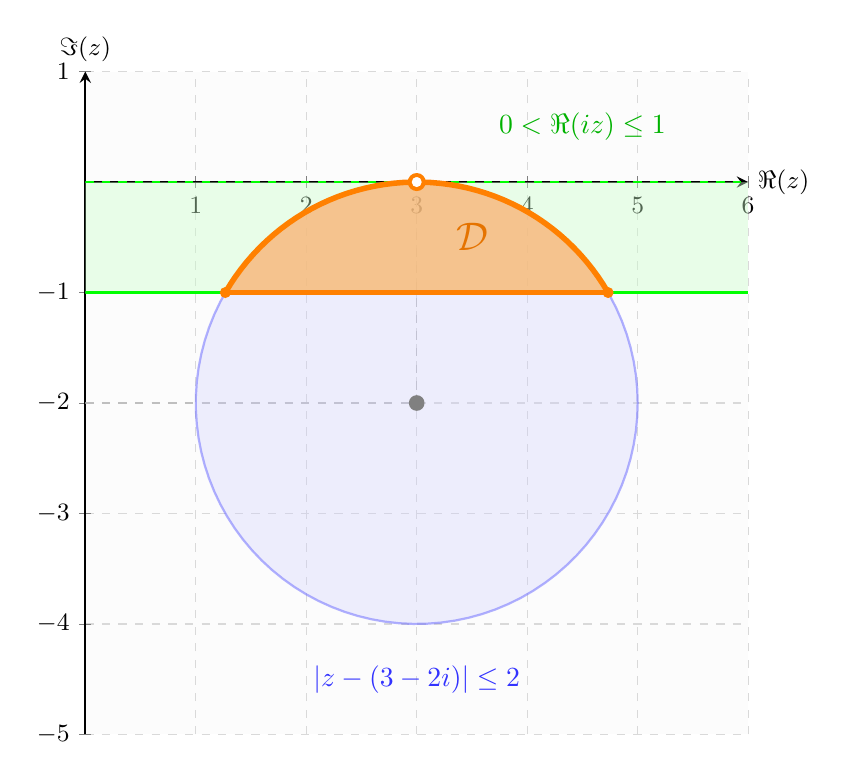
\begin{tikzpicture}
    \begin{axis}[
        width=10cm, height=10cm,
        axis lines=middle,
        axis line style={thick, black},
        xlabel=$\Re(z)$,
        ylabel=$\Im(z)$,
        xlabel style={right},
        ylabel style={above},
        xmin=0, xmax=6,
        ymin=-5, ymax=1,
        xtick={0,1,...,6},
        ytick={-5,-4,...,1},
        grid=major,
        grid style={dashed, gray!30},
        axis background/.style={fill=gray!2},
        tick label style={font=\small},
        label style={font=\small}
    ]

    \draw[dashed, gray!50] (axis cs:3,0) -- (axis cs:3,-2);
    \draw[dashed, gray!50] (axis cs:0,-2) -- (axis cs:3,-2);

    \fill[green!20, opacity=0.4] (axis cs:0,-1) rectangle (axis cs:6,0);

    \addplot [fill=blue!20, draw=blue!60, thick, 
              fill opacity=0.3, draw opacity=0.5,
              domain=0:360, samples=100,
              variable=\t] 
        ({3+2*cos(\t)}, {-2+2*sin(\t)});

    \begin{scope}
    \clip plot[domain=0:360, samples=100, variable=\t] 
        ({3+2*cos(\t)}, {-2+2*sin(\t)});

    \fill[orange!60, opacity=0.7] (axis cs:0,-1) rectangle (axis cs:6,0);
    \end{scope}

    \draw[green, thick] (axis cs:0,-1) -- (axis cs:6,-1);
    \draw[green, thick, dashed] (axis cs:0,0) -- (axis cs:6,0);

    \draw[orange, line width=2pt] 
        plot[domain=30:150, samples=50, variable=\t] 
        ({3+2*cos(\t)}, {-2+2*sin(\t)});

    \draw[orange, line width=2pt] (axis cs:1.268,-1) -- (axis cs:4.732,-1);

    \draw[line width=1.5pt, orange] (axis cs:3,0) circle [radius=2.5pt];
    \fill[white] (axis cs:3,0) circle [radius=1.8pt];

    \fill[orange] (axis cs:1.268,-1) circle [radius=2pt];
    \fill[orange] (axis cs:4.732,-1) circle [radius=2pt];

    \node[circle, fill=gray, inner sep=2pt] at (axis cs:3,-2) {};

    \node[orange!90!black, align=center, font=\Large] at (axis cs:3.5,-0.5) {$\mathcal{D}$};

    \node[blue!80, align=center] at (axis cs:3,-4.5) {$|z-(3-2i)| \leq 2$};
    \node[green!70!black, align=center] at (axis cs:4.5,0.5) 
        {$0 < \Re(iz) \leq 1$};

    \end{axis}
    \end{tikzpicture}
  \end{center}
\end{solution}